\documentclass{jhwhw}
\usepackage[utf8]{inputenc}
\usepackage{amsmath}
\usepackage{amssymb}
\usepackage{braket}
\usepackage{tikz}
\usepackage{forest}
\usepackage{booktabs}
\usepackage{color,soul}
\usepackage{enumitem}
\usepackage{adjustbox}
\usepackage[spanish]{babel}
\newcommand{\subscript}[2]{$#1 _ #2$}
\newcommand{\mytitle}{Act 3.2 Lexer}
\usepackage{graphicx}

\begin{document}

\author{Juan Pablo Salazar-A01740200}
\title{\mytitle}

\maketitle
\begin{center}
    Automata principal
\end{center}
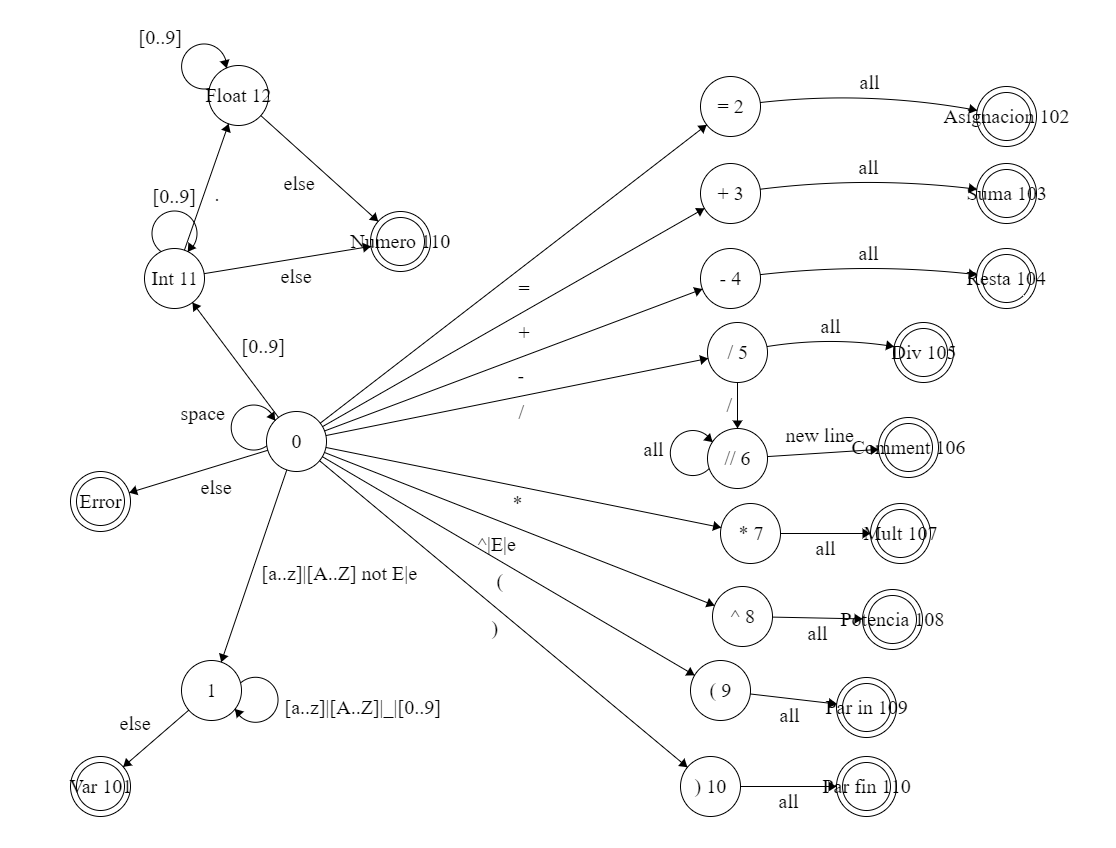
\includegraphics[width = \textwidth]{Act3-2imgs/Automata.png}

\bigskip

El codigo pasa por cada letra con un estado inicial (empieza en 0) y va generando una lista de estados, que finalmente se junta con los caracteres introducidos para hacer los tokens.

\bigskip
El razonamiento detras de este automata es que despues de que llega a un punto final,lo agrega a una lista, vuelve al inicio, que es 0 en este caso, y vuelve a calcular el estado y lo mete a la lista.

\bigskip

Otra cosa es que el codigo analiza linea por linea, asi que se le agrega un espacio al final de cada linea para que el ultimo caracter pueda tener un estado final, ya que cuando se sacan las lineas de haskell se pierden los finales de linea.

Despues de calcular los estados se quita un valor antes del estado final, para marcar que el caracter que esta en esa posicion es el final de un token.

Despues se separan los tokens con los estados finales, entre cada estado final hay un token que termina en un estado final y empieza despues de un estado final.

Para correr el programa nada mas se ocupa compilar con ghc, correrlo e introducir el nombre del archivo a escanear

\$ ghc lexer.hs -o lexer.exe \#windows

\$ ghc lexer.hs -o lexer \#linux

\$./lexer.exe \#windows

\$./lexer \#linux

nombre-archivo.txt

\bigskip

Ejemplo:

Input:  ''a=b+c''
Se analiza: ''a=b+c ''
Estados iniciales: 

[1,101,2,102,1,101,3,103,1,101,0]

Estados despues de quitar valores antes del ultimo: 

[101,102,101,103,101]

Tokens conseguidos:
[(''a'',101),(''='',102),(''b'',101),(''+'',103),(''c'',101)]

\bigskip
Despues de conseguir los tokens con sus estados finales nada mas se convierten en texto para que se regrese como valor final un string con todos los valores.
\end{document}
